% Provenance (never printed): old premiere S material on plate kinematics (rigid
% plates, rates from magnetic anomalies and from satellite positioning, hotspots
% and the Hawaiian chain, the coherence of the model); see
% sources/book2/PROVENANCE.md. Velocities from the NNR-MORVEL56 poles
% (figdata/grade-11/plate_velocities.py), station series from the Nevada Geodetic
% Laboratory (gnss_series.py), volcano ages from Clague and Dalrymple 1987
% (hawaii_chain.py). Euler poles and triple junctions belong to Year 1: the
% rotation pole is told, not defined.
\chapter{प्लेटें और उनकी गतियाँ}\label{ch:g11:plate-motions}

हवाई द्वीप पर मौना की के शिखर के पास, चट्टान में जड़ा एक ऐंटेना
अक्टूबर 1996 से हर दिन स्थिति-निर्धारण उपग्रहों के संकेत ग्रहण कर रहा है।
हर दिन एक कंप्यूटर कुछ मिलीमीटर की सटीकता तक निकालता है कि ऐंटेना कहाँ है।
तीस वर्षों की स्थितियाँ हर वर्ष एक ही कहानी कहती हैं: ऐंटेना,
पर्वत और पूरा द्वीप प्रति वर्ष लगभग \qty{7}{cm} पश्चिम-उत्तर-पश्चिम की ओर
चलते हैं, बिना रुके और बिना मुड़े। 2026 तक ऐंटेना
अपने आरंभिक स्थान से दो मीटर से अधिक दूर था। यह अध्याय
ऐसी गतियों को मापता है, दिखाता है कि वे गोले पर कैसे आपस में मेल खाती हैं, और वही
गति मृत ज्वालामुखियों की उस श्रृंखला में पढ़ता है जो हवाई से उत्तरी प्रशांत
के आर-पार फैली है।
% ledger: data:b2-ngl-gnss

\begin{recall}
\omterm{def:g11:lithosphere-asthenosphere:lithosphere}{स्थलमंडल} विवर्तनिक प्लेटों में टूटा है, जो एक-दूसरे के सापेक्ष
प्रति वर्ष कुछ सेंटीमीटर चलती हैं; उनकी सीमाएँ कटक, खाइयाँ,
टक्कर-क्षेत्र और रूपांतर भ्रंश हैं (पुस्तक 1, कक्षा 7)। तप्त स्थल
प्रावार में गहरा एक स्थान है जो अपने ऊपर की प्लेट पर एक ज्वालामुखी को पोषित करता है; प्लेट
ज्वालामुखी को दूर ले जाती है जबकि तप्त स्थल के ऊपर एक नया ज्वालामुखी बढ़ता है (पुस्तक 1,
कक्षा 7)। स्थिति-निर्धारण उपग्रह का अभिग्राही कई उपग्रहों के संकेतों से
अपनी स्थिति निकालता है (पुस्तक 1, कक्षा 9)। महासागर की तली की चुंबकीय धारियाँ
किसी कटक की \omterm{def:g11:drift-to-spreading:spreading-rate}{प्रसरण दर} देती हैं
(\cref{ch:g11:drift-to-spreading}), और \omterm{def:g11:lithosphere-asthenosphere:lithosphere}{स्थलमंडल} पृथ्वी का कठोर बाहरी
कवच है, लगभग \qty{100}{km} मोटा
(\cref{ch:g11:lithosphere-asthenosphere})। प्रति वर्ष \qty{1}{cm} की चाल
प्रति मिलियन वर्ष \qty{10}{km} है, और प्रति वर्ष \qty{1}{mm} प्रति
मिलियन वर्ष \qty{1}{km} है।
\end{recall}

\begin{omfigure}
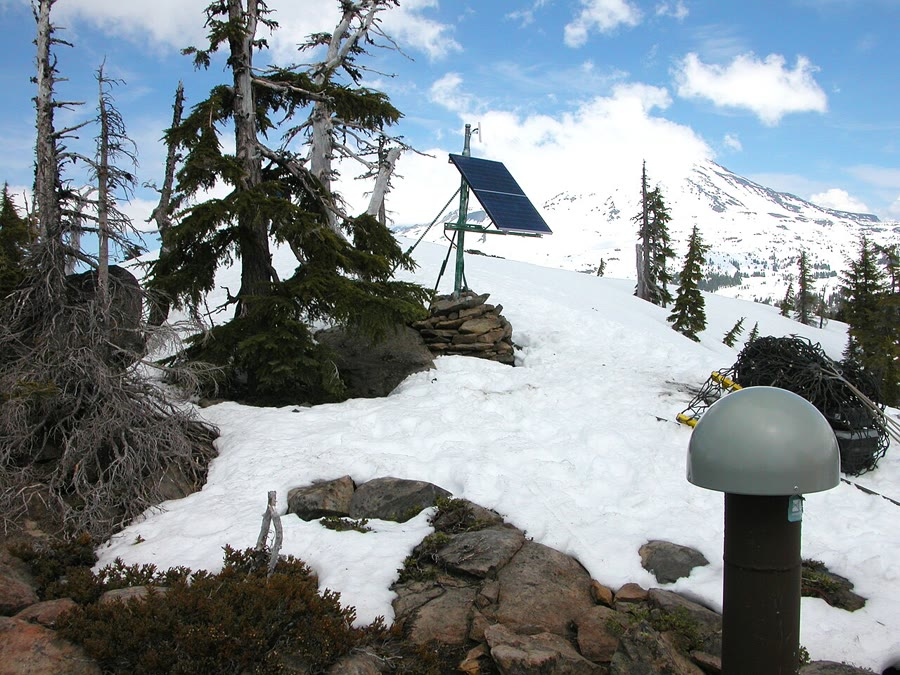
\includegraphics[width=0.62\linewidth]{images/book2/g11-usgs-gps-station.jpg}

{\small ओरेगन की कैस्केड श्रेणी में एक ज्वालामुखी पर एक स्थायी उपग्रह-स्थिति-निर्धारण स्टेशन
(2007)। ऐंटेना धूसर गुंबद के नीचे है, ज़मीन में मज़बूती से गड़े एक
मस्तूल पर; पीछे का सौर पैनल अभिग्राही को ऊर्जा देता है। ऐसा
स्टेशन दिन-प्रतिदिन अपनी स्थिति दर्ज करता है। फ़ोटो: डेव शेरॉड,
USGS (सार्वजनिक डोमेन)।}
\end{omfigure}
% ledger: photo:g11-gps-station

\section{गोले पर दृढ़ प्लेटें}

भूकंप पृथ्वी पर यादृच्छिक रूप से बिखरे नहीं हैं: उनमें से लगभग सभी
संकरी पट्टियों के अनुदिश होते हैं, जो प्लेट-सीमाएँ हैं (पुस्तक 1, कक्षा 7)। प्लेट के
भीतर चट्टान मुश्किल से ही टूटती है। इसलिए प्लेट कोई कोमल खाल नहीं है जो
चलते हुए खिंचती और सिकुड़ती है, बल्कि \omterm{def:g11:lithosphere-asthenosphere:lithosphere}{स्थलमंडल} का एक कड़ा टुकड़ा है जो
एक इकाई के रूप में चलता है।

\begin{definition}[दृढ़ प्लेट]\label{def:g11:plate-motions:rigid-plate}
\emph{दृढ़ प्लेट}\index{दृढ़ प्लेट} \omterm{def:g11:lithosphere-asthenosphere:lithosphere}{स्थलमंडल} का ऐसा टुकड़ा है जो
एक ही खंड के रूप में चलता है: उस पर के बिंदुओं के बीच की दूरियाँ नहीं बदलतीं, और उसका
विरूपण उसकी सीमाओं के अनुदिश संकरे क्षेत्रों में इकट्ठा रहता है।
\end{definition}

दृढ़-प्लेट मॉडल एक सन्निकटन है। कुछ क्षेत्र सैकड़ों
किलोमीटर तक विरूपित होते हैं, जैसे हिमालय के पीछे के ऊँचे पठार या
उत्तरी अमेरिका का पश्चिम, और मॉडल उन्हें चौड़ी सीमाएँ मानता है। पर
पृथ्वी की सतह के अधिकांश भाग पर वह उल्लेखनीय रूप से अच्छा काम करता है: वह
\omterm{def:g11:plate-motions:rigid-plate}{दृढ़ प्लेटों} के लिए जो वेग पूर्वानुमानित करता है, वे उपग्रह स्टेशनों द्वारा मापे गए वेगों से प्रति वर्ष कुछ
मिलीमीटर के भीतर मेल खाते हैं (\cref{sec:g11:plate-motions:predictive}), जबकि प्लेटें
एक-दूसरे के सापेक्ष प्रति वर्ष सेंटीमीटरों चलती हैं।

कोई दृढ़ टोपी गोले की सतह पर कैसे चल सकती है? वह किसी सीधी
रेखा में नहीं सरक सकती, क्योंकि सीधी रेखा गोले को छोड़ देती है। दृढ़ टोपी की
गति चाहे जो हो, वह पृथ्वी के केंद्र से होकर जाने वाले अक्ष के परितः एक \emph{घूर्णन} है।
यह अक्ष सतह से प्लेट के \emph{घूर्णन ध्रुव} पर मिलता है। प्लेट का
कोई बिंदु उस ध्रुव के चारों ओर एक लघु वृत्त के अनुदिश चलता है, और वह
ध्रुव से जितना दूर होता है, उसका वृत्त उतना बड़ा होता है और वह उतना तेज़ चलता है
(नीचे का चित्र)। इस बात का प्रमाण कि दृढ़ टोपी की हर
गति ऐसा ही घूर्णन है, और प्लेट-सीमाओं के वर्णन में घूर्णन ध्रुवों का उपयोग,
पुस्तक~3 के विषय हैं; यहाँ केवल चालों का उपयोग होता है।

\begin{omfigure}
\begin{tikzpicture}[scale=1.15, font=\footnotesize]
  \fill[omSea!45] (0,0) circle (2);
  \draw (0,0) circle (2);
  % small circles about the rotation pole (pole at the top), seen slightly from above
  \foreach \a/\len in {60/0.75, 35/1.23, 0/1.5} {
    \pgfmathsetmacro{\r}{2*cos(\a)}
    \pgfmathsetmacro{\h}{2*sin(\a)}
    \draw[black!45, densely dashed] (-\r,\h) arc[start angle=180, end angle=0, x radius=\r, y radius=0.22*\r];
    \draw[omDef!80!black, line width=0.7pt] (-\r,\h) arc[start angle=180, end angle=360, x radius=\r, y radius=0.22*\r];
    \draw[-{Stealth[length=5pt]}, omProp, line width=1.1pt] (0,\h-0.22*\r) -- ++(\len,0);
  }
  \draw[black!70, dash pattern=on 3pt off 2pt] (0,-2.5) -- (0,2.55);
  \fill (0,2) circle (1.6pt);
  \node[anchor=south west] at (0.05,2.02) {घूर्णन ध्रुव};
  \node[anchor=north, text=black!70] at (0,-2.5) {घूर्णन अक्ष, केंद्र से होकर};
  \fill (0,0) circle (1pt);
  \node[anchor=west, align=left] at (2.25,0.9) {हर बिंदु ध्रुव के\\चारों ओर एक लघु वृत्त\\के अनुदिश चलता है};
  \node[anchor=west, align=left, text=omProp] at (2.25,-0.4) {चाल: ध्रुव से \ang{90}\\पर सबसे अधिक};
\end{tikzpicture}

{\small गोले पर एक \omterm{def:g11:plate-motions:rigid-plate}{दृढ़ प्लेट} पृथ्वी के केंद्र से होकर जाने वाले अक्ष के परितः घूमती है।
घूर्णन ध्रुव के पास के बिंदु लघु वृत्तों के अनुदिश धीरे चलते हैं;
ध्रुव से \ang{90} पर के बिंदु सबसे तेज़ चलते हैं (तीर: पैमाने पर चालें)।}
\end{omfigure}

किसी बिंदु की चाल आसानी से निकाली जा सकती है। ध्रुव से कोणीय दूरी
$\theta$ पर स्थित बिंदु अक्ष से दूरी $R\sin\theta$ पर है, जहाँ
$R = \qty{6371}{km}$ पृथ्वी की त्रिज्या है। यदि प्लेट प्रति मिलियन वर्ष $\omega$
अंश घूमती है, तो बिंदु एक मिलियन वर्ष में भिन्न $\omega/360$ जितना चक्कर लगाता है, उस
वृत्त का जिसकी त्रिज्या $R\sin\theta$ है:
\[
  v = \frac{\omega}{360} \times 2\pi R\sin\theta
    = \frac{\pi\,\omega}{180}\,R\sin\theta .
\]
प्रति मिलियन वर्ष $\omega = \qty{1}{\degree}$ और $\theta = \ang{90}$ के लिए
यह $\pi \times 6371/180 \approx \qty{111}{km}$ प्रति मिलियन वर्ष है,
यानी प्रति वर्ष \qty{11.1}{cm}। इसलिए किसी प्लेट की कोई एक चाल नहीं होती: उसके बिंदु
ऐसी चालों से चलते हैं जो घूर्णन ध्रुव पर शून्य से (यदि ध्रुव
प्लेट पर हो) उससे \ang{90} पर अधिकतम तक होती हैं। किसी कटक के अनुदिश के रूपांतर भ्रंश,
जो दो प्लेटों को एक-दूसरे के पास से सरकने देते हैं, दोनों प्लेटों के सापेक्ष घूर्णन के
ध्रुव के चारों ओर लघु वृत्तों के अनुदिश चलते हैं।
% ledger: earth:Rmean (shared), nnr56:poles

घूर्णन ध्रुवों के प्रकाशित समुच्चय हर प्लेट के लिए उसके
ध्रुव की स्थिति और उसके घूमने की दर देते हैं। उनमें से एक, जो मुख्यतः कटकों के अनुदिश मापी गई
\omterm{def:g11:drift-to-spreading:spreading-rate}{प्रसरण दरों} और प्रसरण दिशाओं से बना है, 56
प्लेटों का वर्णन करता है; प्रशांत प्लेट प्रति मिलियन वर्ष
\ang{0.651} घूमती है, यूरेशियाई प्लेट \ang{0.223}। इन
संख्याओं से एक कंप्यूटर किसी भी प्लेट के किसी भी बिंदु का वेग निकालता है
(नीचे का मानचित्र)।
% ledger: nnr56:poles, nnr56:data

\begin{omfigure}
\begin{tikzpicture}
\begin{axis}[ommap, width=\linewidth, xtick={-180,-90,...,180}, ytick={-60,0,60}]
\addplot[fill=omLithAlluv, draw=black!45, line width=0.2pt] table {figdata/out/shared-geo-land.dat};
\addplot[omRidge, line width=0.6pt] table {figdata/out/shared-geo-school-ridge.dat};
\addplot[omRidge!70!black, line width=0.6pt] table {figdata/out/shared-geo-school-transform.dat};
\addplot[omTrench, line width=0.6pt] table {figdata/out/shared-geo-school-subduction.dat};
\addplot[fill=omTrench, draw=none] table {figdata/out/shared-geo-school-teeth.dat};
\addplot[black!65, line width=0.6pt] table {figdata/out/shared-geo-school-collision.dat};
% computed in figdata/grade-11/plate_velocities.py (NNR-MORVEL56); 2.5 degrees per cm/yr
\addplot[black, line width=0.8pt, -{Stealth[length=4pt]}, quiver={u=\thisrow{dx}, v=\thisrow{dy}}]
  table[x=lon, y=lat] {figdata/out/grade-11-plate_velocities-arrows.dat};
\addplot[omProp, line width=1.2pt, -{Stealth[length=5pt]}, quiver={u=\thisrow{dx}, v=\thisrow{dy}}]
  table[x=lon, y=lat] {figdata/out/grade-11-plate_velocities-hawaii.dat};
\addplot[only marks, mark=*, mark size=1.3pt, omProp] coordinates {(-155.46,19.80)};
\node[font=\scriptsize, anchor=north, fill=white, fill opacity=0.75, text opacity=1, inner sep=1pt]
  at (axis cs:-150,15) {मौना की};
\draw[black, line width=0.8pt, -{Stealth[length=4pt]}] (axis cs:-172,-80) -- (axis cs:-147,-80);
\node[font=\scriptsize, anchor=west, fill=white, fill opacity=0.75, text opacity=1, inner sep=1pt]
  at (axis cs:-145,-80) {प्रति वर्ष \qty{10}{cm}};
\end{axis}
\end{tikzpicture}

{\small 16 प्लेटों के भीतर के बिंदुओं के वेग, उनके
प्रकाशित घूर्णन ध्रुवों से परिकलित, ऐसे निर्देश-तंत्र में जिसमें \omterm{def:g11:lithosphere-asthenosphere:lithosphere}{स्थलमंडल} समग्र रूप से
नहीं घूमता। प्रशांत, नाज़्का, कोकोस, ऑस्ट्रेलियाई और भारतीय प्लेटें सबसे तेज़ चलती हैं;
यूरेशियाई, उत्तर और दक्षिण अमेरिकी तथा अंटार्कटिक प्लेटें धीरे। लाल तीर:
मौना की पर प्रशांत प्लेट। घूर्णन ध्रुव: आर्गस, गॉर्डन और डीमेट्स
(2011); प्लेट-सीमाएँ: बर्ड (2003); स्थल: नैचुरल अर्थ।}
\end{omfigure}
% ledger: nnr56:poles, data:pb2002, data:ne-land

\section{गतियों का मापन}

\subsection{चाल मापने के दो ढंग}

महासागर की तली की चुंबकीय धारियाँ वह चाल देती हैं जिससे दो प्लेटें
किसी कटक के आर-पार एक-दूसरे से दूर होती हैं (\cref{ch:g11:drift-to-spreading}): कटक-अक्ष से किसी धारी की
दूरी को उसकी आयु से भाग दीजिए। मिली हुई चाल धारी की आयु पर, प्रायः
पिछले कुछ मिलियन वर्षों पर, औसत होती है, और वह
\emph{सापेक्ष} चाल है, एक प्लेट की, दूसरी से देखी गई। धारियाँ
उन प्लेटों के बारे में कुछ नहीं बतातीं जो किसी खाई या टक्कर-क्षेत्र पर मिलती हैं, क्योंकि वहाँ
कोई महासागरीय तली नहीं बनती।

उपग्रह-स्थिति-निर्धारण आज के एक अकेले बिंदु की गति मापता है, कुछ
वर्षों या दशकों में। स्थायी स्टेशन ठोस चट्टान में जड़ा होता है, जिससे
वह प्लेट के साथ चलता है; उसकी दैनिक स्थितियाँ, समय के सापेक्ष आलेखित करने पर,
एक सरल रेखा के अनुदिश सजती हैं जिसकी ढाल स्टेशन का वेग है।

\begin{method}[स्थिति-निर्धारण की समय-श्रेणी से दर]\label{met:g11:plate-motions:rate}
\begin{enumerate}
  \item स्टेशन की पूर्व-स्थिति और उत्तर-स्थिति को समय के सापेक्ष
        आलेखित कीजिए, दो आलेखों पर या एक ही आलेख पर।
  \item वह सरल रेखा खींचिए जो हर श्रेणी का सबसे अच्छा अनुसरण करती है (या उस पर दूर-दूर के दो
        बिंदु पढ़िए)। उसकी ढाल, मिलीमीटर प्रति वर्ष में,
        पूर्व-चाल $v_E$ या उत्तर-चाल $v_N$ है; पश्चिम या
        दक्षिण की ओर चलने वाले स्टेशन की चाल ऋणात्मक होती है।
  \item स्टेशन की चाल $v = \sqrt{v_E^2 + v_N^2}$ है; उसकी दिशा
        पूर्व--पश्चिम रेखा से ऐसा कोण $\alpha$ बनाती है कि
        $\tan\alpha = |v_N|/|v_E|$, उत्तर की ओर यदि $v_N > 0$ और
        पूर्व की ओर यदि $v_E > 0$।
\end{enumerate}
\end{method}

\begin{omfigure}
\begin{tikzpicture}
\begin{axis}[ompt, name=a, width=0.5\linewidth, height=5.6cm, xmin=1995, xmax=2027, ymin=-200, ymax=120,
  xlabel={वर्ष}, ylabel={स्थिति (\unit{cm})}, xtick={2000,2010,2020},
  xticklabel style={/pgf/number format/set thousands separator={}},
  title={\small मौना की, हवाई (MKEA)}, tick label style={font=\scriptsize}]
% computed in figdata/grade-11/gnss_series.py; ledger: data:b2-ngl-gnss
\addplot[only marks, mark=*, mark size=0.5pt, omDef] table[x=year, y=north] {figdata/out/grade-11-gnss_series-mkea.dat};
\addplot[only marks, mark=*, mark size=0.5pt, omProp] table[x=year, y=east] {figdata/out/grade-11-gnss_series-mkea.dat};
\node[font=\scriptsize, text=omDef!80!black, anchor=west] at (axis cs:1996.5,80) {उत्तर};
\node[font=\scriptsize, text=omProp!80!black, anchor=west] at (axis cs:1996.5,-120) {पूर्व};
\end{axis}
\begin{axis}[ompt, at={(a.east)}, anchor=west, xshift=0.9cm, width=0.5\linewidth, height=5.6cm, xmin=1995, xmax=2027,
  ymin=-10, ymax=70, xlabel={वर्ष}, xtick={2000,2010,2020},
  xticklabel style={/pgf/number format/set thousands separator={}},
  title={\small वेत्ज़ेल, जर्मनी (WTZR)}, tick label style={font=\scriptsize}]
\addplot[only marks, mark=*, mark size=0.5pt, omDef] table[x=year, y=north] {figdata/out/grade-11-gnss_series-wtzr.dat};
\addplot[only marks, mark=*, mark size=0.5pt, omProp] table[x=year, y=east] {figdata/out/grade-11-gnss_series-wtzr.dat};
\node[font=\scriptsize, text=omDef!80!black, anchor=west] at (axis cs:2014,22) {उत्तर};
\node[font=\scriptsize, text=omProp!80!black, anchor=west] at (axis cs:2006,40) {पूर्व};
\end{axis}
\end{tikzpicture}

{\small दो स्थायी स्टेशनों की मासिक माध्य स्थितियाँ, उनके
पहले महीने से मापी गई: पूर्व (लाल) और उत्तर (नीला)। हर श्रेणी एक
सरल रेखा के अनुदिश सजती है, जिसकी ढाल उस दिशा में स्टेशन की चाल है। प्रशांत प्लेट पर स्थित मौना की पश्चिम और उत्तर की ओर चलता है; यूरेशियाई प्लेट पर स्थित
वेत्ज़ेल पूर्व और उत्तर की ओर, लगभग तीन गुना धीरे। आँकड़े:
नेवादा भूगणितीय प्रयोगशाला (ब्लेविट, हैमंड और क्रीमर, 2018)।}
\end{omfigure}
% ledger: data:b2-ngl-gnss

\begin{example}[मौना की का स्टेशन]\label{ex:g11:plate-motions:mkea}
अक्टूबर 1996 से सितंबर 2026 तक मौना की स्टेशन की मासिक स्थितियाँ
दो सरल रेखाओं का अनुसरण करती हैं, जिनकी ढालें $v_E =
\qty{-63.2}{mm}$ प्रति वर्ष (पश्चिम की ओर) और $v_N = \qty{+34.5}{mm}$ प्रति वर्ष हैं।
चाल $\sqrt{63.2^2 + 34.5^2} \approx \qty{72}{mm}$ प्रति वर्ष है, और $\tan\alpha
= 34.5/63.2 \approx 0.546$ से $\alpha \approx \ang{29}$ मिलता है: स्टेशन
प्रति वर्ष \qty{7.2}{cm} पश्चिम से \ang{29} उत्तर की दिशा में चलता है। प्रशांत प्लेट का घूर्णन ध्रुव
इस स्थान पर प्रति वर्ष \qty{6.9}{cm}, पश्चिम से \ang{28} उत्तर, का पूर्वानुमान
देता है।
\end{example}
% ledger: data:b2-ngl-gnss, nnr56:poles (prediction computed in plate_velocities.py)

बिंदु रेखाओं के आसपास कुछ मिलीमीटर बिखरे हैं, जो एक वर्ष की
गति से बहुत कम है: कुछ वर्षों के मापन के बाद किसी
स्टेशन का वेग प्रति वर्ष एक मिलीमीटर से बेहतर सटीकता से ज्ञात हो जाता है।

\subsection{सापेक्ष और निरपेक्ष गति}

वेग हमेशा किसी चीज़ के सापेक्ष मापा जाता है। मौना की
स्टेशन पूरी पृथ्वी से जुड़े निर्देश-तंत्र के सापेक्ष प्रति वर्ष \qty{7.2}{cm} चलता है;
उत्तरी अमेरिका के किसी स्टेशन से देखने पर, जो स्वयं चलता है, उसका
वेग भिन्न है।

\begin{definition}[सापेक्ष गति; निरपेक्ष गति]\label{def:g11:plate-motions:relative-motion}
प्लेट $A$ की, प्लेट $B$ के सापेक्ष, \emph{सापेक्ष गति}\index{सापेक्ष गति}
उसकी वह गति है जो $B$ पर खड़े प्रेक्षक को दिखती है।
किसी प्लेट की \emph{निरपेक्ष गति}\index{निरपेक्ष गति} उसकी वह गति है
जो गहरी पृथ्वी से जुड़े निर्देश-तंत्र के सापेक्ष हो, उदाहरण के लिए स्थिर माने गए
तप्त स्थलों का एक समुच्चय, या वह निर्देश-तंत्र जिसमें \omterm{def:g11:lithosphere-asthenosphere:lithosphere}{स्थलमंडल} समग्र रूप से
नहीं घूमता।
\end{definition}

कटक, खाइयाँ और रूपांतर भ्रंश \omterm{def:g11:plate-motions:relative-motion}{सापेक्ष गतियों} से आकार लेते हैं: किसी सीमा पर
यह मायने रखता है कि दोनों प्लेटें एक-दूसरे के सापेक्ष कैसे चलती हैं।
सापेक्ष वेग उन विस्थापनों की तरह जुड़ते हैं जो वे उत्पन्न करते हैं।

\begin{proposition}[सापेक्ष वेग तीरों की तरह जुड़ते हैं]\label{prop:g11:plate-motions:sum}
मान लीजिए $\vec v_{A/B}$ प्लेट $A$ का, प्लेट $B$ के सापेक्ष, सीमा के
किसी दिए हुए बिंदु पर वेग है, और इसी तरह दूसरे युग्मों के लिए। किन्हीं भी तीन
प्लेटों $A$, $B$, $C$ के लिए,
\[
  \vec v_{A/C} = \vec v_{A/B} + \vec v_{B/C},
  \qquad\text{और}\qquad
  \vec v_{B/A} = -\vec v_{A/B}.
\]
\end{proposition}

\begin{proof}
थोड़े समय $\Delta t$ में, मान लीजिए $A$ से जुड़ा एक बिंदु स्थिति $P$
से $P'$ तक जाता है, जैसा $C$ से दिखता है, और $B$ का वह बिंदु जो $P$ पर था,
$Q$ तक जाता है, जैसा $C$ से दिखता है। $B$ से देखने पर $A$ का बिंदु $Q$ से
$P'$ तक गया है। विस्थापन सदिशों की तरह जुड़ते हैं:
$\overrightarrow{PP'} = \overrightarrow{PQ} + \overrightarrow{QP'}$, यानी
$A$ का $C$ से देखा गया विस्थापन = $B$ का $C$ से देखा गया विस्थापन +
$A$ का $B$ से देखा गया विस्थापन। $\Delta t$ से भाग देने पर $\vec v_{A/C}
= \vec v_{B/C} + \vec v_{A/B}$ मिलता है। $C = A$ लेने पर बायाँ पक्ष शून्य है: $\vec
v_{B/A} = -\vec v_{A/B}$।
\end{proof}

\begin{method}[वेग-त्रिभुज को बंद करना]\label{met:g11:plate-motions:triangle}
\begin{enumerate}
  \item हर ज्ञात वेग को उसके पूर्व और उत्तर घटकों के साथ लिखिए, सभी
        एक ही बिंदु पर मापे गए।
  \item $\vec v_{A/B}$ ज्ञात करने के लिए, $A$ और $B$ के एक ही
        निर्देश-तंत्र $C$ में वेगों से, घटाइए: $\vec v_{A/B} = \vec v_{A/C} - \vec v_{B/C}$,
        घटक-दर-घटक।
  \item किसी चित्र पर $\vec v_{A/C}$ और $\vec v_{B/C}$ की पूँछें
        एक ही बिंदु पर रखिए: $\vec v_{B/C}$ के सिरे से
        $\vec v_{A/C}$ के सिरे तक का तीर $\vec v_{A/B}$ है, और वह त्रिभुज को बंद करता है।
  \item उसकी लंबाई और दिशा
        \cref{met:g11:plate-motions:rate} की तरह परिकलित कीजिए।
\end{enumerate}
\end{method}

\begin{example}[सैन एंड्रियास भ्रंश]\label{ex:g11:plate-motions:san-andreas}
मध्य कैलिफ़ोर्निया में, \ang{35.5} उत्तर और \ang{120.5} पश्चिम पर, घूर्णन
ध्रुव प्रशांत प्लेट को वेग $(-42.1, +26.4)$ और उत्तर
अमेरिकी प्लेट को $(-11.9, -14.8)$ देते हैं, मिलीमीटर प्रति वर्ष में (पूर्व, उत्तर), पूरे
\omterm{def:g11:lithosphere-asthenosphere:lithosphere}{स्थलमंडल} के निर्देश-तंत्र में। उत्तरी अमेरिका के सापेक्ष प्रशांत प्लेट
$(-42.1 + 11.9,\ 26.4 + 14.8) = (-30.2, +41.2)$ से चलती है, यानी
$\sqrt{30.2^2 + 41.2^2} \approx \qty{51}{mm}$ प्रति वर्ष, उत्तर से
\ang{36} पश्चिम की दिशा में (नीचे का चित्र)। सैन
एंड्रियास भ्रंश, जो उत्तर-पश्चिम की ओर चलता है, इस सरकन का अधिकांश भाग वहन करता है।
\end{example}
% ledger: nnr56:poles (computed in plate_velocities.py: relative pa/na at 120.5 W 35.5 N)

\begin{omfigure}
\begin{tikzpicture}[x=0.065cm, y=0.065cm, font=\footnotesize]
  % mm/yr, from plate_velocities.py: PA (-42.1, 26.4), NA (-11.9, -14.8), PA/NA (-30.2, 41.2)
  \draw[black!25] (-8,0) -- (8,0) (0,-8) -- (0,8);
  \draw[-{Stealth[length=5pt]}, omProp, line width=1.1pt] (0,0) -- (-42.1,26.4)
    node[pos=0.55, above right, inner sep=1pt] {$\vec v_{\mathrm{PA}}$};
  \draw[-{Stealth[length=5pt]}, omDef, line width=1.1pt] (0,0) -- (-11.9,-14.8)
    node[pos=0.8, right=2pt] {$\vec v_{\mathrm{NA}}$};
  \draw[-{Stealth[length=5pt]}, black, line width=1.1pt] (-11.9,-14.8) -- (-42.1,26.4)
    node[pos=0.4, left=9pt, align=right] {$\vec v_{\mathrm{PA/NA}}$\\प्रति वर्ष \qty{51}{mm}};
  \fill (0,0) circle (0.9pt);
  % compass
  \draw[-{Stealth[length=4pt]}] (25,10) -- (25,24) node[above] {उ};
  \draw[-{Stealth[length=4pt]}] (25,10) -- (39,10) node[right] {पू};
  \draw (25,-18) -- (40.4,-18);
  \node[below] at (32.7,-18) {प्रति वर्ष \qty{20}{mm}};
  \draw (25,-17) -- (25,-19) (40.4,-17) -- (40.4,-19);
\end{tikzpicture}

{\small मध्य कैलिफ़ोर्निया में एक वेग-त्रिभुज को बंद करना (पैमाने पर)। लाल:
प्रशांत प्लेट; नीला: उत्तर अमेरिकी प्लेट, दोनों पूरे
\omterm{def:g11:lithosphere-asthenosphere:lithosphere}{स्थलमंडल} के निर्देश-तंत्र में। काला: उत्तरी अमेरिका से देखी गई प्रशांत प्लेट,
नीले तीर के सिरे से लाल तीर के सिरे तक का तीर।}
\end{omfigure}

\section{तप्त स्थल पथ}

\subsection{स्थिर प्लूम के ऊपर एक प्लेट}

हवाई प्रशांत प्लेट के बीच में है, निकटतम प्लेट-सीमा से
\qty{3000}{km} से अधिक दूर।
% ledger: usgs:hawaii-hotspot (Book 1 row)
 इसके ज्वालामुखियों को एक तप्त स्थल पोषित करता है (पुस्तक~1,
कक्षा~7)। प्लेट उसके ऊपर से चलती है, और हर ज्वालामुखी
तप्त स्थल से दूर ले जाया जाता है जबकि उसके पीछे एक नया ज्वालामुखी बढ़ता है।

\begin{definition}[तप्त स्थल पथ]\label{def:g11:plate-motions:hotspot-track}
\emph{तप्त स्थल पथ}\index{तप्त स्थल पथ} ज्वालामुखियों की, और
समुद्री पर्वत कहलाने वाले डूबे ज्वालामुखियों की, वह पंक्ति है जिसे कोई प्लेट
किसी तप्त स्थल के ऊपर से चलते हुए उससे दूर ले जाती है: सक्रिय ज्वालामुखी तप्त स्थल के ऊपर होता है, और
ज्वालामुखी उससे दूरी के साथ अधिकाधिक पुराने होते जाते हैं।
\end{definition}

\begin{omfigure}
\begin{tikzpicture}[font=\footnotesize]
  % plate moving to the left over a fixed plume (not to scale)
  \fill[omSea!50] (0,0) rectangle (11,0.9);
  \fill[black!22] (0,-0.9) rectangle (11,0);
  \draw (0,0) -- (11,0);
  \draw[densely dashed] (0,0.9) -- (11,0.9) node[right] {समुद्र-तल};
  \node[anchor=east] at (10.95,-0.45) {स्थलमंडल};
  \fill[omLithPeridotite!40] (0,-2.3) rectangle (11,-0.9);
  \node[anchor=west] at (0.1,-1.6) {दुर्बलतामंडल};
  % plume
  \fill[omProp!55] (8.6,-2.3) -- (8.6,-1.2) .. controls (8.6,-0.9) and (9.2,-0.9) .. (9.2,-1.2) -- (9.2,-2.3) -- cycle;
  \fill[omProp!55] (8.75,-0.95) rectangle (9.05,0);
  \node[anchor=north, align=center] at (8.9,-2.35) {प्लूम, प्रावार में स्थिर};
  % volcanoes: active over the plume, older ones carried left, eroded and sunk
  \fill[black!65] (8.0,0) -- (8.9,1.6) -- (9.8,0) -- cycle;
  \fill[black!55] (5.4,0) -- (6.2,1.15) -- (7.0,0) -- cycle;
  \fill[black!50] (3.0,0) -- (3.55,0.62) -- (3.85,0.62) -- (4.4,0) -- cycle;
  \fill[black!45] (0.8,0) -- (1.25,0.42) -- (1.65,0.42) -- (2.1,0) -- cycle;
  \node[above] at (8.9,1.6) {सक्रिय};
  \node[above] at (6.2,1.15) {$t_1$};
  \node[above] at (3.7,0.62) {$t_2$};
  \node[above] at (1.45,0.42) {$t_3$};
  % plate motion
  \draw[-{Stealth[length=6pt]}, line width=1.2pt] (6.5,-0.45) -- (4.0,-0.45) node[left] {प्लेट चलती है, चाल $v$};
  % distance d = v t
  \draw[{Stealth[length=4pt]}-{Stealth[length=4pt]}] (3.7,2.3) -- (8.9,2.3) node[midway, above] {$d_2 = v\,t_2$};
  \draw[black!50] (3.7,1.05) -- (3.7,2.4) (8.9,2.0) -- (8.9,2.4);
\end{tikzpicture}

{\small प्रावार में स्थिर प्लूम के ऊपर चाल $v$ से चलती एक प्लेट (पैमाने पर
नहीं)। प्लूम के ऊपर बना आयु $t$ का ज्वालामुखी
दूरी $d = v\,t$ तक ले जाया गया है; पुराने ज्वालामुखी अपरदित होकर
समुद्र के नीचे डूब जाते हैं।}
\end{omfigure}

\begin{proposition}[तप्त स्थल पथ से चाल]\label{prop:g11:plate-motions:hotspot}
यदि कोई तप्त स्थल गहरे प्रावार में स्थिर रहता है और उसके ऊपर की प्लेट
नियत चाल $v$ से नियत दिशा में चलती है, तो जो ज्वालामुखी
समय $t$ पहले तप्त स्थल के ऊपर था, वह अब पथ के अनुदिश सक्रिय ज्वालामुखी से
इस दूरी पर है:
\[
  d = v\,t
\]
ज्वालामुखियों की आयु, उनकी दूरियों के सापेक्ष आलेखित करने पर,
मूल-बिंदु से होकर जाने वाली ऐसी सरल रेखा पर पड़ती हैं जिसकी
ढाल $1/v$ है, और $v$ प्लेट की निरपेक्ष चाल है।
\end{proposition}

\begin{proof}
ज्वालामुखी वहाँ बना जहाँ प्लेट तप्त स्थल के ऊपर थी, और तब से वह
प्लेट के साथ चला है। समय $t$ में प्लेट एक नियत दिशा में
$v\,t$ चली है, इसलिए ज्वालामुखी प्लेट के उस बिंदु से, जो अब तप्त स्थल के ऊपर है और जहाँ
सक्रिय ज्वालामुखी है, उतनी दूरी पर है। संबंध
$t = d/v$ मूल-बिंदु से होकर जाने वाली ढाल
$1/v$ की सरल रेखा का है। चाल तप्त स्थल के सापेक्ष, यानी गहरे प्रावार के
सापेक्ष, मापी जाती है: यह निरपेक्ष चाल है।
\end{proof}

\subsection{हवाई--सम्राट श्रृंखला}

हवाई द्वीप से द्वीपों, प्रवाल-भित्तियों और समुद्री पर्वतों की एक पंक्ति लगभग
\qty{3400}{km} पश्चिम-उत्तर-पश्चिम की ओर जाती है, फिर तीखा मोड़ लेकर
सम्राट समुद्री पर्वतों के रूप में उत्तर की ओर जारी रहती है --- अकेला सुइको समुद्री पर्वत
किलाउआ से \qty{4860}{km} पर है --- और कामचटका तथा
अल्यूशियन के पास की खाइयों तक पहुँचती है (नीचे का चित्र)।
% ledger: cd87:ages

\begin{omfigure}
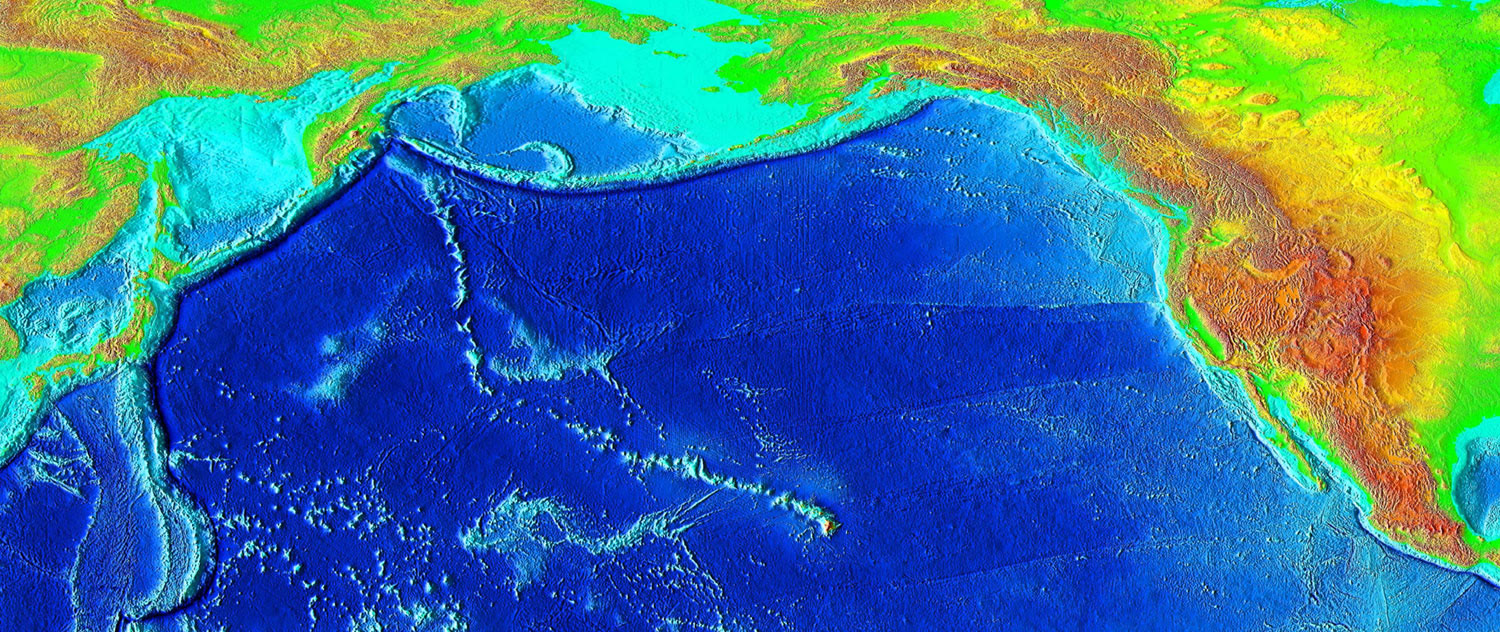
\includegraphics[width=\linewidth]{images/book2/g11-ngdc-hawaii-chain.jpg}

{\small उत्तरी प्रशांत की तली का छायांकित उच्चावच। हवाई श्रृंखला
हवाई द्वीप (नीचे बीच में, भूरा) से
पश्चिम-उत्तर-पश्चिम की ओर जाती है; मोड़ पर वह उत्तर की ओर मुड़कर सम्राट समुद्री पर्वतों में बदल जाती है, जो
कामचटका और अल्यूशियन के अनुदिश की खाई पर समाप्त होते हैं। चित्र: राष्ट्रीय
भूभौतिकीय आँकड़ा केंद्र, NOAA (सार्वजनिक डोमेन)।}
\end{omfigure}
% ledger: photo:g11-hawaii-chain

श्रृंखला के 37 ज्वालामुखियों के लावाओं का पोटैशियम--आर्गन काल-निर्धारण, जो
द्वीपों पर एकत्र किए गए, समुद्री पर्वतों से खुरचकर निकाले गए या उनके अवसादों को भेदकर वेधित किए गए,
उनकी आयु देता है (नीचे का आलेख)। मौना की लगभग
\num{0.4} मिलियन वर्ष पुराना है, काउआई \num{5.1}, मिडवे \num{27.7}, और
सम्राट श्रृंखला के दूर के सिरे के पास का सुइको समुद्री पर्वत \num{64.7}। आयु
सक्रिय ज्वालामुखी किलाउआ से दूरी के साथ बढ़ती है, जैसा \omterm{def:g11:plate-motions:hotspot-track}{तप्त स्थल पथ}
पूर्वानुमानित करता है।
% ledger: cd87:ages

\begin{omfigure}
\begin{tikzpicture}
\begin{axis}[ompt, width=0.82\linewidth, height=6.4cm, xmin=0, xmax=5000, ymin=0, ymax=70,
  xlabel={श्रृंखला के अनुदिश किलाउआ से दूरी (\unit{km})}, ylabel={आयु (मिलियन वर्ष)},
  xticklabel style={/pgf/number format/set thousands separator={}},
  legend style={font=\scriptsize, at={(0.03,0.97)}, anchor=north west}, legend cell align=left]
% computed in figdata/grade-11/hawaii_chain.py; ledger: cd87:ages
\addplot[only marks, mark=o, mark size=1.6pt, omDef, error bars/.cd, y dir=both, y explicit]
  table[x=dist, y=age, y error=err] {figdata/out/grade-11-hawaii_chain-hawaiian.dat};
\addplot[only marks, mark=triangle, mark size=2pt, omProp, error bars/.cd, y dir=both, y explicit]
  table[x=dist, y=age, y error=err] {figdata/out/grade-11-hawaii_chain-emperor.dat};
\addplot[black, densely dashed, line width=0.6pt] table[x=dist, y=age] {figdata/out/grade-11-hawaii_chain-fit.dat};
\legend{हवाई श्रृंखला, मोड़ और सम्राट श्रृंखला, {मूल-बिंदु से होकर रेखा, प्रति वर्ष \qty{9.1}{cm}}}
\draw[black!50, densely dotted] (axis cs:3400,0) -- (axis cs:3400,70);
\node[font=\scriptsize, anchor=south, rotate=90] at (axis cs:3400,8) {मोड़};
\node[font=\scriptsize, anchor=north west] at (axis cs:519,5.1) {काउआई};
\node[font=\scriptsize, anchor=south] at (axis cs:2432,30) {मिडवे};
\node[font=\scriptsize, anchor=south east] at (axis cs:4860,65.5) {सुइको};
\end{axis}
\end{tikzpicture}

{\small हवाई--सम्राट श्रृंखला के ज्वालामुखियों की आयु, किलाउआ से उनकी
दूरी के सापेक्ष, आयुओं की अनिश्चितताओं के साथ।
हवाई श्रृंखला के अनुदिश बिंदु मूल-बिंदु से होकर जाने वाली सरल रेखा का अनुसरण करते हैं;
मोड़ के आगे आयु दूरी के साथ अधिक तेज़ी से बढ़ती है। आँकड़े: क्लैग और डैलरिम्पल
(1987)।}
\end{omfigure}

हवाई श्रृंखला के अनुदिश, लगभग \qty{3300}{km} तक, बिंदु
मूल-बिंदु से होकर जाने वाली एक सरल रेखा के आसपास बिखरे हैं। इस भाग के 26
काल-निर्धारित ज्वालामुखियों से सबसे अच्छा मेल खाने वाली रेखा हर
\qty{91}{km} पर एक मिलियन वर्ष बढ़ती है: \cref{prop:g11:plate-motions:hotspot} के अनुसार, प्रशांत प्लेट
तप्त स्थल के ऊपर से लगभग \qty{91}{km} प्रति मिलियन वर्ष, यानी प्रति वर्ष \qty{9.1}{cm},
चली है। आयुओं के लेखकों ने पूरी श्रृंखला को अपने ढंग से मिलाकर
प्रति वर्ष \qty{8.6}{cm} पाया।
% ledger: cd87:ages (fit computed in hawaii_chain.py), cd87:rate

मोड़ के आगे आयु दूरी के साथ अधिक तेज़ी से बढ़ती है: सम्राट
श्रृंखला के अनुदिश प्लेट अधिक धीरे चली, औसतन प्रति वर्ष लगभग \qty{6.5}{cm}
(नौ काल-निर्धारित समुद्री पर्वतों से होकर सबसे अच्छी सरल रेखा)। और श्रृंखला
दिशा बदलती है। यदि तप्त स्थल अपनी जगह पर रहा, तो मोड़ प्रशांत प्लेट की गति की
दिशा में परिवर्तन अंकित करता है। नई आयु
मोड़ का आरंभ किम्मेई समुद्री पर्वत के पास, लगभग 50 मिलियन वर्ष
पहले, रखती हैं, उसी समय जब प्रशांत के प्रसरण-कटकों का पुनर्गठन हुआ
और उसके पश्चिमी किनारे के अनुदिश द्वीप-चापों के पहले ज्वालामुखी बने:
प्लेट ने अपना मार्ग बदला।
% ledger: cd87:ages (Emperor fit computed in hawaii_chain.py), sc06:bend

\section{मॉडल की पूर्वानुमान-शक्ति}\label{sec:g11:plate-motions:predictive}

प्लेट मॉडल कहता है कि कुछ \omterm{def:g11:plate-motions:rigid-plate}{दृढ़ प्लेटें} अपने घूर्णन ध्रुवों के परितः घूमती हैं,
और लगभग सब कुछ उनकी सीमाओं पर होता है। इसकी शक्ति यह है कि
पूरी तरह अलग-अलग विधियों से, समय की बहुत अलग-अलग
अवधियों में किए गए मापन एक ही उत्तर देते हैं।

\begin{itemize}
  \item \emph{भूकंप और ज्वालामुखी} सीमाओं के अनुदिश इकट्ठा होते हैं, और
        सीमा का प्रकार उनका प्रकार पूर्वानुमानित करता है: कटकों के अनुदिश उथले भूकंप,
        गहरे भूकंप केवल खाइयों के पास (\cref{ch:g11:subduction-zones})।
  \item \emph{महासागरीय तली} कटकों के अनुदिश सबसे नई है और उनसे दूर अधिकाधिक
        पुरानी, दोनों ओर सममित रूप से
        (\cref{ch:g11:drift-to-spreading})।
  \item \emph{पर्वत-पट्टियाँ} वहाँ उठती हैं जहाँ प्लेटें अभिसरित होती हैं: भारत अब भी
        हिमालय के आर-पार प्रति वर्ष लगभग \qty{4.5}{cm} की दर से यूरेशिया की ओर चलता है,
        जैसा घूर्णन ध्रुवों से परिकलित है (\cref{ch:g12:mountain-building})।
  \item \emph{विधियों में चालें मेल खाती हैं}: नीचे की तालिका
        उपग्रह-स्थिति-निर्धारण द्वारा आज मापी गई चालों की तुलना
        घूर्णन ध्रुवों द्वारा पूर्वानुमानित चालों से करती है, जिनकी \omterm{def:g11:drift-to-spreading:spreading-rate}{प्रसरण दरें} मुख्यतः
        चुंबकीय धारियों से आती हैं और पिछले \num{0.8} से \num{3.2} मिलियन वर्षों की
        गति का औसत लेती हैं, और उस चाल से भी जो
        कोई \omterm{def:g11:plate-motions:hotspot-track}{तप्त स्थल पथ} दसियों मिलियन वर्षों में अंकित करता है।
\end{itemize}
% ledger: nnr56:poles, nnr56:data (India-Eurasia computed in plate_velocities.py at 85 E 28 N)

\begin{center}
\small
\begin{tabular}{|l|c|c|}
\hline
क्या मापा गया & विधि & चाल (प्रति वर्ष \unit{cm}) \\ \hline
मौना की, प्रशांत प्लेट & उपग्रह-स्थिति-निर्धारण, 30 वर्ष & 7.2 \\
मौना की, प्रशांत प्लेट & घूर्णन ध्रुव & 6.9 \\
वेत्ज़ेल, यूरेशियाई प्लेट & उपग्रह-स्थिति-निर्धारण, 31 वर्ष & 2.6 \\
वेत्ज़ेल, यूरेशियाई प्लेट & घूर्णन ध्रुव & 2.3 \\
हवाई तप्त स्थल के ऊपर प्रशांत प्लेट & ज्वालामुखियों की आयु, 40 मिलियन वर्ष & 9.1 \\ \hline
\end{tabular}
\end{center}
% ledger: data:b2-ngl-gnss, nnr56:poles, cd87:ages (all computed in figdata/grade-11)

घूर्णन-ध्रुव चालें और स्टेशन-चालें प्रति वर्ष
\qty{0.3}{cm} के भीतर मेल खाती हैं, यद्यपि पहली चालें मिलियनों वर्षों का औसत हैं और
दूसरी केवल दशकों का: प्लेटें आज वैसे ही चलती हैं जैसे वे मिलियनों
वर्षों से चली हैं। तप्त स्थल-चाल अधिक है: वह एक दूसरे निर्देश-तंत्र में, स्वयं
तप्त स्थल के निर्देश-तंत्र में, और कहीं अधिक लंबे समय में मापी जाती है।

पूरी प्लेटों की चालों की तुलना करने पर एक और प्रतिरूप दिखता है। सबसे
तेज़ चलने वाली प्लेटों --- कोकोस, नाज़्का, प्रशांत, ऑस्ट्रेलियाई और फ़िलिपीन
सागर --- सभी का एक लंबा किनारा किसी खाई पर प्रावार में डूबता है; उनकी माध्य
चालें औसतन प्रति वर्ष लगभग \qty{6.5}{cm} हैं। ऐसे किनारे के बिना वाली
प्लेटें, जिनमें यूरेशियाई, उत्तर और दक्षिण अमेरिकी, अफ़्रीकी और
अंटार्कटिक प्लेटें हैं, औसतन प्रति वर्ष लगभग \qty{2.4}{cm} चलती हैं। प्लेटों को क्या
चलाता है, इसका यह सुराग \cref{ch:g11:subduction-zones} में उठाया गया है।
% ledger: nnr56:rms (means computed in plate_velocities.py)

\section{अभ्यास}

\begin{exercise}[$\star$]\label{exo:g11:plate-motions:1}
\omterm{def:g11:plate-motions:rigid-plate}{दृढ़ प्लेट} की परिभाषा दीजिए। \omterm{def:g11:lithosphere-asthenosphere:lithosphere}{स्थलमंडल} का विरूपण कहाँ इकट्ठा रहता है,
और कौन-सा रोज़मर्रा का भूकंपीय प्रेक्षण यह दिखाता है?
\end{exercise}

\begin{exercise}[$\star$]\label{exo:g11:plate-motions:2}
मौना की स्टेशन प्रति वर्ष \qty{72}{mm} चलता है। इस चाल को
किलोमीटर प्रति मिलियन वर्ष में व्यक्त कीजिए। स्टेशन 30 वर्षों में कितनी दूर चलता है?
एक मिलियन वर्षों में?
\end{exercise}

\begin{exercise}[$\star$]\label{exo:g11:plate-motions:3}
दस वर्षों में एक स्टेशन \qty{30}{cm} पूर्व और \qty{40}{cm} उत्तर की ओर चला।
उसकी पूर्व और उत्तर चालें, उसकी चाल, और उसकी दिशा का उत्तर से बना
कोण ज्ञात कीजिए।
\end{exercise}

\begin{exercise}[$\star$]\label{exo:g11:plate-motions:4}
\omterm{def:g11:plate-motions:hotspot-track}{तप्त स्थल पथ} की परिभाषा दीजिए। हवाई श्रृंखला के अनुदिश सबसे नया
ज्वालामुखी कहाँ है, और आयु किस दिशा में बढ़ती है? इससे
प्रशांत प्लेट के चलने की दिशा के बारे में क्या पता चलता है?
\end{exercise}

\begin{exercise}[$\star$]\label{exo:g11:plate-motions:5}
काउआई श्रृंखला के अनुदिश किलाउआ से \qty{519}{km} पर है, और उसके सबसे पुराने लावा
\num{5.1} मिलियन वर्ष पुराने हैं। तप्त स्थल को स्थिर मानकर बताइए कि प्लेट उसे
किस औसत चाल से ले गई है, किलोमीटर प्रति मिलियन वर्ष में और
सेंटीमीटर प्रति वर्ष में?
\end{exercise}

\begin{exercise}[$\star\star$]\label{exo:g11:plate-motions:6}
दोनों स्टेशन-श्रेणियों के आलेख में, वेत्ज़ेल स्टेशन 31 वर्षों में लगभग
\qty{63}{cm} पूर्व और \qty{48}{cm} उत्तर की ओर चला। उसकी पूर्व और उत्तर
चालें, उसकी चाल, और उसकी दिशा ज्ञात कीजिए। उसकी चाल की तुलना मौना
की की चाल से कीजिए।
\end{exercise}

\begin{exercise}[$\star\star$]\label{exo:g11:plate-motions:7}
आइसलैंड में, \ang{64.5} उत्तर और \ang{18} पश्चिम पर, घूर्णन ध्रुव
उत्तर अमेरिकी प्लेट को वेग $(-10.5, +20.6)$ और यूरेशियाई
प्लेट को $(+7.7, +16.3)$ देते हैं, मिलीमीटर प्रति वर्ष में (पूर्व, उत्तर)। (1)
यूरेशिया के सापेक्ष उत्तरी अमेरिका का वेग, उसकी चाल और उसकी दिशा ज्ञात कीजिए।
(2) आइसलैंड को पार करने वाले कटक के लिए यह चाल क्या है? (3) इसकी तुलना
उत्तरी अटलांटिक के लिए प्रायः उद्धृत प्रति वर्ष \qty{2}{cm} की दर से कीजिए।
\end{exercise}

\begin{exercise}[$\star\star$]\label{exo:g11:plate-motions:8}
प्रशांत प्लेट प्रति मिलियन वर्ष \ang{0.651} घूमती है। (1) उसके घूर्णन ध्रुव से
\ang{90} पर स्थित बिंदु की चाल, सेंटीमीटर प्रति वर्ष में, ज्ञात कीजिए। (2) और
ध्रुव से \ang{30} पर स्थित बिंदु की? (3) प्लेट पर चाल कहाँ शून्य होती है? क्या
पूरी प्लेट की चाल एक संख्या से दी जा सकती है?
\end{exercise}

\begin{exercise}[$\star\star$]\label{exo:g11:plate-motions:9}
हिमालय के उत्तर में, \ang{28} उत्तर और \ang{85} पूर्व पर, घूर्णन ध्रुव
भारतीय प्लेट को वेग $(+40.6, +38.6)$ और यूरेशियाई प्लेट को
$(+24.0, -3.3)$ देते हैं, मिलीमीटर प्रति वर्ष में (पूर्व, उत्तर)। (1) यूरेशिया के सापेक्ष
भारत का वेग, उसकी चाल और उसकी दिशा ज्ञात कीजिए। (2) यदि यह
वैसा ही रहे, तो 10 मिलियन वर्षों में दोनों प्लेटें कितनी अभिसरित होंगी?
\end{exercise}

\begin{exercise}[$\star\star$]\label{exo:g11:plate-motions:10}
नेकर किलाउआ से \qty{1058}{km} पर है और \num{10.3} मिलियन वर्ष पुराना है;
मिडवे \qty{2432}{km} दूर है और \num{27.7} मिलियन वर्ष पुराना है। दोनों ज्वालामुखियों के
बनने के समयों के बीच तप्त स्थल के ऊपर प्लेट की चाल ज्ञात कीजिए।
प्रति वर्ष \qty{9.1}{cm} से तुलना कीजिए।
\end{exercise}

\begin{exercise}[$\star\star$]\label{exo:g11:plate-motions:11}
किसी बिंदु पर प्लेट $A$, प्लेट $B$ के सापेक्ष, प्रति वर्ष \qty{3}{cm} पूर्व की ओर चलती है,
और प्लेट $B$, प्लेट $C$ के सापेक्ष, प्रति वर्ष \qty{4}{cm} उत्तर की ओर चलती है।
(1) वेग-त्रिभुज बनाइए और $A$ का, $C$ के सापेक्ष, वेग ज्ञात कीजिए:
चाल और दिशा। (2) $C$ का, $A$ के सापेक्ष, वेग क्या है?
\end{exercise}

\begin{exercise}[$\star\star\star$]\label{exo:g11:plate-motions:12}
मौना की किलाउआ से \qty{54}{km} पर है और \num{0.375} मिलियन वर्ष
पुराना है। (1) यह प्लेट के लिए कौन-सी चाल देता है? (2) एक ज्वालामुखी कुछ दसियों
किलोमीटर चौड़ा होता है, और वह कई लाख वर्षों तक बढ़ता है। मान लीजिए
तप्त स्थल से उसकी दूरी \qty{25}{km} तक अनिश्चित है: तब चाल किन
मानों के बीच है? (3) समझाइए कि तप्त स्थल के पास के नए ज्वालामुखी
चाल का खराब अनुमान क्यों देते हैं, और उससे दूर के ज्वालामुखी
बेहतर क्यों हैं।
\end{exercise}

\begin{exercise}[$\star\star\star$]\label{exo:g11:plate-motions:13}
किसी स्टेशन की मासिक स्थितियाँ अपनी सरल रेखा के आसपास लगभग \qty{5}{mm} बिखरी हैं।
कोई गति तब स्पष्ट दिखती है जब वह बिखराव के दस गुने से अधिक हो जाए।
(1) मौना की स्टेशन की गति, प्रति वर्ष \qty{72}{mm}, स्पष्ट देखने के लिए कितने समय तक
मापना होगा? (2) और प्रति वर्ष \qty{5}{mm} की गति के लिए, जैसी
किसी महाद्वीप के भीतर धीरे-धीरे विरूपित होते क्षेत्र के आर-पार होती है? (3) उपग्रहों के उन्हें माप पाने से
बहुत पहले ही प्लेटों की चालें चुंबकीय धारियों से क्यों
मापी गईं?
\end{exercise}

\begin{exercise}[$\star\star\star$]\label{exo:g11:plate-motions:14}
\ang{30} दक्षिण (\ang{13.5} पश्चिम) पर मध्य-अटलांटिक कटक पर घूर्णन
ध्रुव दक्षिण अमेरिकी प्लेट को वेग $(-4.9, +11.0)$ और
अफ़्रीकी प्लेट को $(+27.1, +17.9)$ देते हैं, मिलीमीटर प्रति वर्ष में (पूर्व, उत्तर)।
(1) अफ़्रीका के सापेक्ष दक्षिण अमेरिका का वेग, उसकी चाल और उसकी
दिशा ज्ञात कीजिए। (2) कटक की पूर्ण और अर्ध \omterm{def:g11:drift-to-spreading:spreading-rate}{प्रसरण दरें} निकालिए।
(3) दक्षिण अटलांटिक के अवसादों ने पिछले 66 मिलियन वर्षों पर औसत लगभग प्रति वर्ष \qty{1.9}{cm}
की अर्ध दर दी
(\cref{ch:g11:drift-to-spreading})। तुलना कीजिए, और सुझाइए कि इस अंतर का
क्या अर्थ हो सकता है।
\end{exercise}

\begin{exercise}[$\star\star\star$]\label{exo:g11:plate-motions:15}
एक स्टेशन प्रति वर्ष \qty{20}{mm} पूर्व की ओर स्थिर रूप से चलता है। मापन के दस
वर्षों के ठीक बीच में एक भूकंप उसे एकाएक \qty{50}{mm}
पश्चिम की ओर खिसका देता है। (1) समय के सापेक्ष उसकी पूर्व-स्थिति का रेखाचित्र बनाइए। (2) केवल
पहली और अंतिम स्थितियों से कौन-सी चाल मिलती? (3) श्रेणी के
दोनों आधे भाग, अलग-अलग, कौन-सी चाल देते हैं? (4) भूगणितज्ञ को ऐसे
उछाल से कैसे निपटना चाहिए?
\end{exercise}

\section{समस्या: हवाई--सम्राट श्रृंखला को पढ़ना}

\begin{problem}[{सप्ताहांत समस्या --- ज्वालामुखियों में लिखी एक प्लेट की चाल}]
\label{pb:g11:plate-motions:1}
% values from Clague and Dalrymple 1987, Table 1.4 (ledger cd87:ages); fits computed in
% figdata/grade-11/hawaii_chain.py (v_hawaiian 91.2, v_emperor_free 64.6); bend sc06:bend;
% MKEA rates data:b2-ngl-gnss
तालिका हवाई--सम्राट श्रृंखला के तेरह ज्वालामुखियों की, श्रृंखला के अनुदिश मापी गई, किलाउआ से दूरी और
पोटैशियम--आर्गन आयु देती है।
किलाउआ तप्त स्थल के ऊपर का सक्रिय ज्वालामुखी है; मोड़ ऐबट
और दाइकाकुजी के बीच है।

\begin{center}
\small
\begin{tabular}{|l|c|c||l|c|c|}
\hline
ज्वालामुखी & दूरी (\unit{km}) & आयु (\unit{Ma}) & ज्वालामुखी & दूरी (\unit{km}) & आयु (\unit{Ma}) \\ \hline
मौना की & 54 & 0.375 & ऐबट & 3280 & 38.7 \\ \hline
काउआई & 519 & 5.1 & दाइकाकुजी & 3493 & 42.4 \\ \hline
निहोआ & 780 & 7.2 & कोको (दक्षिण) & 3758 & 48.1 \\ \hline
नेकर & 1058 & 10.3 & ओजिन & 4102 & 55.2 \\ \hline
लेसन & 1818 & 19.9 & निन्तोकू & 4452 & 56.2 \\ \hline
मिडवे & 2432 & 27.7 & सुइको (केंद्र) & 4860 & 64.7 \\ \hline
कोलाहान & 3128 & 38.6 & & & \\ \hline
\end{tabular}
\end{center}

\medskip
\noindent\textbf{भाग I --- आयु और दूरियाँ।}
\begin{enumerate}
  \item तालिका का कौन-सा ज्वालामुखी सबसे नया है, और कौन-सा सबसे पुराना? श्रृंखला के अनुदिश
        आयु कैसे बदलती है?
  \item दिखाइए कि किलोमीटर में दूरी को मिलियन वर्षों में आयु से भाग देने पर
        मिलीमीटर प्रति वर्ष में चाल मिलती है।
  \item काउआई द्वारा दी गई औसत चाल $d/t$ परिकलित कीजिए।
  \item नेकर, लेसन, मिडवे, कोलाहान और ऐबट के लिए $d/t$ परिकलित कीजिए।
  \item तालिका के उन आठ ज्वालामुखियों के लिए, जो मोड़ से पहले हैं, आयु को दूरी के सापेक्ष
        आलेखित कीजिए। क्या बिंदु मूल-बिंदु से होकर जाने वाली किसी सरल रेखा के
        निकट हैं?
\end{enumerate}

\medskip
\noindent\textbf{भाग II --- तप्त स्थल के ऊपर प्लेट की चाल।}
\begin{enumerate}[resume]
  \item समझाइए कि स्थिर तप्त स्थल और नियत
        चाल $v$ से चलती प्लेट के लिए आयु $t$ और दूरी $d$ क्यों $t = d/v$ को संतुष्ट करती हैं।
  \item प्रश्न~4 की पाँच चालों का माध्य परिकलित कीजिए।
  \item हवाई श्रृंखला के सभी 26 काल-निर्धारित ज्वालामुखियों से सबसे अच्छा मेल खाने वाली,
        मूल-बिंदु से होकर जाने वाली सरल रेखा \qty{91}{km} प्रति मिलियन वर्ष देती है।
        प्रश्न~7 से तुलना कीजिए।
  \item इस चाल से प्लेट को काउआई को तप्त स्थल से उसके वर्तमान स्थान तक
        ले जाने में कितना समय लगता? उसकी आयु से तुलना कीजिए।
  \item प्रशांत प्लेट तप्त स्थल के ऊपर से किस दिशा में चलती है?
\end{enumerate}

\medskip
\noindent\textbf{भाग III --- मोड़।}
\begin{enumerate}[resume]
  \item दाइकाकुजी और सुइको (केंद्र) के बनने के समयों के बीच प्लेट की औसत चाल
        परिकलित कीजिए।
  \item दाइकाकुजी से आगे के नौ काल-निर्धारित ज्वालामुखियों से होकर सबसे अच्छी सरल रेखा
        \qty{65}{km} प्रति मिलियन वर्ष देती है। इसकी तुलना
        हवाई श्रृंखला के अनुदिश की चाल से कीजिए।
  \item नई आयु मोड़ का आरंभ किलाउआ से \qty{3668}{km} दूर किम्मेई
        समुद्री पर्वत के पास, लगभग 50 मिलियन वर्ष पहले, रखती हैं।
        इससे पूरी हवाई श्रृंखला के लिए कौन-सी औसत चाल मिलती है?
        \qty{91}{km} प्रति मिलियन वर्ष से तुलना कीजिए, और समझाइए कि दोनों क्यों
        सही हो सकती हैं।
  \item यदि तप्त स्थल स्थिर रहा, तो मोड़ प्रशांत प्लेट के बारे में क्या
        अंकित करता है?
  \item नए काल-निर्धारण ने सम्राट श्रृंखला के अनुदिश चाल में बड़े परिवर्तन पाए,
        पर उसकी दिशा में थोड़ा ही परिवर्तन। समझाइए कि किसी
        श्रृंखला की दिशा और उसकी आयुओं के बीच का अंतराल दो स्वतंत्र
        सूचनाएँ क्यों हैं।
\end{enumerate}

\medskip
\noindent\textbf{भाग IV --- आज के उपग्रह-मापन से तुलना।}
\begin{enumerate}[resume]
  \item मौना की स्टेशन प्रति वर्ष पूर्व की ओर $\qty{-63.2}{mm}$ और
        उत्तर की ओर $\qty{+34.5}{mm}$ चलता है। उसकी चाल और उसकी दिशा ज्ञात कीजिए।
  \item हवाई श्रृंखला किलाउआ से पश्चिम-उत्तर-पश्चिम की ओर जाती है। क्या
        स्टेशन की दिशा इससे संगत है?
  \item स्टेशन प्रति वर्ष \qty{7.2}{cm} देता है, श्रृंखला प्रति वर्ष \qty{9.1}{cm}।
        दो कारण बताइए कि दोनों संख्याओं का बराबर होना क्यों आवश्यक नहीं है।
  \item प्रति मिलियन वर्ष \qty{91}{km} पर प्लेट को मौना की को तप्त स्थल से
        और \qty{100}{km} दूर ले जाने में कितना समय लगेगा?
  \item निष्कर्ष निकालिए: पिछले 40 मिलियन वर्षों में प्रशांत प्लेट हवाई
        तप्त स्थल के ऊपर से किस चाल से चली है?
\end{enumerate}
\end{problem}
